% Vertical line between columns
\documentclass{ctexbeamer}

% Theme choice:
\usetheme{CambridgeUS}

\begin{document}

\begin{frame}{垂直分隔线}
  \begin{columns}
  % Column 1
  \begin{column}{0.49\textwidth}
    \begin{itemize}
      \item Input layer: 2 neurons.
      \item Hidden layer: 5 neurons.
      \item Output layer: 2 neurons.
    \end{itemize}
  \end{column}

  % Column 2 (vertical line)
  \begin{column}{.02\textwidth}
    \rule{.1mm}{0.7\textheight}
  \end{column}

  % Column 3    
  \begin{column}{0.49\textwidth}
    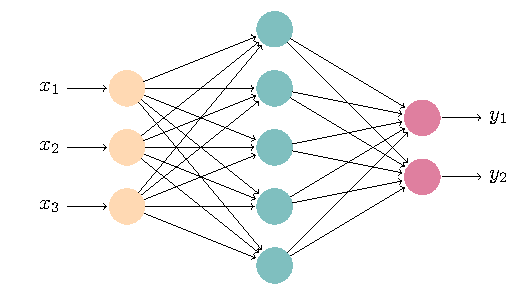
\includegraphics[width=\textwidth]{neural-networks.pdf}
  \end{column}
  \end{columns}
\end{frame}

\end{document}